\newpage
\section{Mengen}

% ------------------------------------------------------------------------------
\subsection{Begriff}
Eine \textbf{Menge} $M$ ist eine Sammlung von unterscheidbaren Objekten, den \textbf{Elementen}. Im unserem Mathematikunterricht handelt es sich bei diesen Objekten um Zahlen. In der höheren Mathematik werden aber auch andere Dinge wie Zahlenpaare, Funktionen oder Mengen in Mengen verpackt.


Mengen werden normalerweise mit Grossbuchstaben bezeichnet, Elemente mit Kleinbuchstaben. Eine Menge $M$ wird grafisch als Kreis dargestellt. Die Elemente $a$, $b$  und $c$ der Menge werden innerhalb des Kreises dargestellt, andere Objekte wie $d$ ausserhalb des Kreises.
\begin{center}
  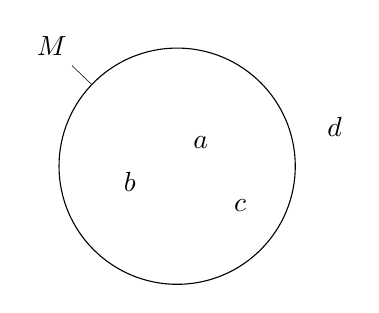
\begin{tikzpicture}[pin distance=0.3cm, pin edge=black]
    \node [draw, circle, minimum size =3cm, pin=above left:$M$] at (0,0) {};
    \node at (0.3, 0.3) {$a$};
    \node at (-0.6, -0.2) {$b$};
    \node at (0.8, -0.5) {$c$};
    \node at (2.0, 0.5) {$d$};
  \end{tikzpicture}
\end{center}
Enthält die Menge $M$ ein Objekt $a$, so wird gesagt, dass $a$ \textbf{ein Element von} $M$ ist und geschrieben:
\[
  a \in M
\]
Enthält die Menge $M$ das Objekt $d$ nicht, so ist $d$ \textbf{kein Element von} $M$. Dies wird so geschrieben:
\[
  d \notin M
\]

% ------------------------------------------------------------------------------
\subsection{Definition durch Aufzählung}
Eine Menge kann durch das Aufzählen aller ihrer Elemente definiert werden. Die Elemente werden durch Strichpunkte getrennt in geschweiften Klammern geschrieben.

Um anzugeben, dass die Menge $M$ aus den Elementen $a$, $b$ und $c$ besteht, wird geschrieben:
\[
  M = \{ a; b; c \}
\]

\begin{note}
\textbf{Hinweis:} Die Elemente werden durch einen Strichpunkt ($;$) getrennt um eine Verwechslung mit dem Dezimalpunkt zu vermeiden. Manchmal werden die Elemente auch durch ein Komma ($,$) oder einen senkrechten Strich ($|$) getrennt.
\end{note}


Wenn nicht alle Elemente hinschreiben werden können, dürfen auch Aufzählungspunkte verwendet werden.

\begin{example}
  \textbf{Beispiel:}  Die Menge der natürlichen Zahlen ist
  \[
    \mathbb{N} = \{0; 1; 2; 3;\ldots \}
  \]
  \textbf{Beispiel:} Die Menge der Dezimalziffern $D$ ist
  \[
    D = \{ 0; 1; 2; \ldots ; 9 \} = \{ 0;1;2;3;4;5;6;7;8;9 \}
  \]
\end{example}

% ------------------------------------------------------------------------------
\subsection{Definition durch Auswahl}

Eine Menge kann auch durch das Auswählen von bestimmten Elementen aus einer anderen Menge definiert werden:
\[
  M = \{ a \in G\mid \text{Eigenschaft von a} \}
\]
Dabei wird in den geschweiften Klammern zuerst angegeben, aus welcher Menge $G$ die Elemente stammen. Nach dem senkrechten Strich wird angegeben, welche Eigenschaft die Elemente $a$ aus $G$ haben müssen, um zu dieser Menge zu gehören.

\begin{example}
  \textbf{Beispiel:} Die Menge der ungeraden Dezimalziffern $U$ kann so definiert werden:
  \[
    U = \{ a \in D \mid a \;\text{ist ungerade} \} = \{ 1; 3; 5; 7; 9 \}
  \]
\end{example}

% ------------------------------------------------------------------------------
\subsection{Gleichheit von Mengen}
Zwei Mengen sind gleich, wenn sie die gleichen Elemente enthalten. Die Reihenfolge der Elemente spielt keine Rolle.
\begin{example}
  \textbf{Beispiele:}
  \[
    \{1;2\} = \{2;1\} \qquad \{1;2;3\} \neq \{1;2\}
  \]
\end{example}

% ------------------------------------------------------------------------------
\subsection{Leere Menge $\{\}$}
Die Menge ohne Elemente heisst \textbf{leere Menge}. Sie wird durch leere geschweifte Klammern dargestellt:
\[
  \{ \}
\]

\begin{note}
  \textbf{Achtung:} Die leere Menge enthält keine Zahl. Sie unterscheidet sich damit von der Menge, welche die Zahl Null enthält:
  \[
    \{\} \neq \{0\}
  \]
\end{note}


% ------------------------------------------------------------------------------
\subsection{Differenzmenge $A \setminus B$}

Die Differenzmenge $A \setminus B$ ist die Menge aller Elemente, welche in $A$, jedoch nicht in $B$ enthalten sind. Achtung: Die Differenzmenge $B \setminus A$ ist eine andere Menge als $A \setminus B$.

\begin{center}
  \begin{minipage}[b]{0.45\textwidth}
    \centering
    \begin{tikzpicture}[pin distance=0.3cm, pin edge=black]
      \fill[lightgreen](-0.9,0) circle(1.5cm);
      \fill[white](0.9,0) circle(1.5cm);
      \node [draw, circle, minimum size =3cm, pin=above left:$A$] at (-0.9,0) {};
      \node [draw, circle, minimum size =3cm, pin=above right:$B$] at (0.9,0) {};
      \node at (-1.4,0) {$A \setminus B$};
     \end{tikzpicture}
  \end{minipage}
  \begin{minipage}[b]{0.45\textwidth}
    \centering
    \begin{tikzpicture}[pin distance=0.3cm, pin edge=black]
      \fill[lightgreen](0.9,0) circle(1.5cm);
      \fill[white](-0.9,0) circle(1.5cm);
      \node [draw, circle, minimum size =3cm, pin=above left:$A$] at (-0.9,0) {};
      \node [draw, circle, minimum size =3cm, pin=above right:$B$] at (0.9,0) {};
      \node at (1.4,0) {$B \setminus A$};
    \end{tikzpicture}
  \end{minipage}
\end{center}

\begin{example}
  \textbf{Beispiel:} Gegeben sind die Menge $A = \{0;1;2;3;4\}$ und die Menge $B = \{0;2;4;6;8\}$. Wir erhalten die Differenzmengen:
  \[
    A \setminus B = \{1;3\} \qquad B \setminus A = \{6;8\}
  \]
\end{example}

% ------------------------------------------------------------------------------
\subsection{Spezielle Zahlenmengen}

Im Skript \textit{Zahlen und Operationen} sind bereits Bezeichnungen für spezielle Zahlenmengen eingeführt worden. Diese werden in der folgenden Tabelle nochmals zusammengefasst:

\begin{center}
  \renewcommand{\arraystretch}{1.3}
  \begin{tabularx}{0.8\textwidth}{Xcl}
      \textbf{Bezeichnung} & \textbf{Symbol} & \textbf{Menge} \\
    \toprule
      natürliche Zahlen    & $\mathbb{N}$    & $\{0, 1, 2, 3, 4, \ldots\}$ \\
    \midrule
      ganze Zahlen         & $\mathbb{Z}$    & $\{\ldots, -2, -1, 0, 1, 2, \ldots\}$ \\
    \midrule
      rationale Zahlen     & $\mathbb{Q}$    & $\left\{\tfrac{z}{n} \;\middle|\; z,n\in\mathbb{Z}, n\neq 0 \right\} $ \\
    \midrule
      reelle Zahlen        & $\mathbb{R}$    & \\
    \bottomrule
  \end{tabularx}
\end{center}

Diesen Symbolen kann ein hochgestelltes Plus oder Minus hinzugefügt werden, um auszudrücken, dass nur die positiven beziehungsweise negativen Zahlen gemeint sind. Mit einer tiefgestellten Null wird ausgedrückt, dass sich auch die Null in der Menge befindet. Dies wird hier anhand der ganzen Zahlen illustriert:
\begin{center}
  \renewcommand{\arraystretch}{1.3}
  \begin{tabularx}{0.8\textwidth}{Xcl}
      \textbf{Bezeichnung}       & \textbf{Symbol}      & \textbf{Menge} \\
    \toprule
      positive ganze Zahlen      & $\mathbb{Z}^{+}$     & $\{1, 2, 3, 4, \ldots\}$ \\
    \midrule
      nichtnegative ganze Zahlen & $\mathbb{Z}_{0}^{+}$ & $\{0, 1, 2, 3, 4, \ldots\}$ \\
    \midrule
      negative ganze Zahlen      & $\mathbb{Z}^{-}$     & $\{\ldots, -4, -3, -2, -1 \}$ \\
    \midrule
      nichtpositive ganze Zahlen & $\mathbb{Z}_{0}^{-}$ & $\{\ldots, -4, -3, -2, -1, 0 \}$ \\
    \bottomrule
  \end{tabularx}
\end{center}

% ------------------------------------------------------------------------------
\subsection{Intervalle}

Die Menge aller reellen Zahlen zwischen zwei bestimmten Zahlen $a$ und $b$ wird als Intervall bezeichnet. $a$ und $b$ sind die Grenzen des Intervalls. Dabei spielt es eine Rolle, ob die Grenze ebenfalls zum Intervall gehört oder nicht. Gehört die Grenze dazu, wird dies als geschlossen bezeichnet. Offen bedeutet, dass die Grenze nicht dazu gehört.

Es werden die folgenden Begriffe und Schreibweisen verwendet:

\begin{center}
  \renewcommand{\arraystretch}{1.1}
  \begin{tabularx}{0.9\textwidth}{XXX}
    \textbf{Begriff} & \textbf{Schreibweise} & \textbf{Definition} \\
  \toprule
    geschlossenes Intervall & $[a, b]$ & $\{ x\in\mathbb{R} \;|\; a \leq x \leq b\}$ \\
  \midrule
    linksoffenes Intervall & $(a, b]$ oder $]a, b]$ & $\{ x\in\mathbb{R} \;|\; a< x \leq b\}$ \\
  \midrule
    rechtsoffenes Intervall & $[a, b)$ oder $[a, b[$ & $\{ x\in\mathbb{R} \;|\; a \leq x < b\}$ \\
  \midrule
    offenes Intervall & $(a, b)$ oder $]a, b[$ & $\{ x\in\mathbb{R} \;|\; a< x < b\}$ \\
  \bottomrule
  \end{tabularx}
\end{center}

Linksoffene und rechtsoffene Intervalle werden zusammen auch als halboffene Intervalle bezeichnet.

% ------------------------------------------------------------------------------
\subsection{Grundmenge $\mathbb{G}$}

Wenn in der Mathematik Probleme gelöst werden, muss zunächst die Menge möglichen Lösungen vorgegeben werden. Diese Menge wird als Grundmenge $\mathbb{G}$ bezeichnet.

In der reinen Mathematik ist die Grundmenge üblicherweise die Menge der reellen Zahlen
\[
  \mathbb{G} = \mathbb{R}
\]
Werden jedoch geometrische oder angewandte Probleme in der Mathematik gelöst, so macht es Sinn, eine andere Grundmenge zu wählen. So ist in der Geometrie eine Länge immer positiv, hier ist also die Grundmenge gleich $\mathbb{R^{+}}$. Werden Dinge gezählt, ist die Grundmenge gleich $\mathbb{N}$.

\begin{example}
  \textbf{Beispiele:} Die Grundmenge für
  \begin{itemize}[noitemsep]
    \item eine Anzahl Personen ist $\mathbb{G} = \mathbb{N}$
    \item die Länge einer Strecke ist $\mathbb{G} = \mathbb{R}^{+}$
    \item einen Kontostand ist $\mathbb{G} =
    \{q \;|\; q\in \mathbb{Q} \;\text{und}\; q\cdot 100 \in \mathbb{Z}\}$
    \item Zeugnisnoten ist $\mathbb{G} = \{1;1.5;2;2.5;3;3.5;4;4.5;5;5.5;6\}$
  \end{itemize}
\end{example}
